\documentclass{beamer}

\usetheme{Pittsburgh}
\useinnertheme{default}
\setbeamertemplate{footline}[page number]
\setbeamertemplate{navigation symbols}{}

%\usepackage[utf8]{inputenc}
\usepackage{listings}
\lstset{ %
language=Ruby,                % choose the language of the code
basicstyle=\footnotesize,       % the size of the fonts that are used for the code
numbers=left,                   % where to put the line-numbers
numberstyle=\footnotesize,      % the size of the fonts that are used for the line-numbers
stepnumber=0,                   % the step between two line-numbers. If it's 1 each line 
                                % will be numbered
numbersep=5pt,                  % how far the line-numbers are from the code
backgroundcolor=\color{white},  % choose the background color. You must add \usepackage{color}
showspaces=false,               % show spaces adding particular underscores
showstringspaces=false,         % underline spaces within strings
showtabs=false,                 % show tabs within strings adding particular underscores
frame=none,	                % adds a frame around the code
tabsize=2,	                % sets default tabsize to 2 spaces
captionpos=b,                   % sets the caption-position to bottom
breaklines=true,                % sets automatic line breaking
breakatwhitespace=false,        % sets if automatic breaks should only happen at whitespace
title=\lstname,                 % show the filename of files included with \lstinputlisting;
                                % also try caption instead of title
escapeinside={\%*}{*)},         % if you want to add a comment within your code
emph={add,output,input,icecast,single,playlist,file,
              fallback,crossfade,http,fade,initial,final,cross},            % if you want to add more keywords to the set
keywordstyle=\color[rgb]{0,0.5,0.3},
emphstyle=\color{red},
stringstyle=\color{blue},
}

\newcommand{\kw}[1]{{\color{red} #1}}

\usepackage{tikz}
\usepackage[all]{xy}

\renewcommand{\emph}[1]{\alert{#1}}
\renewcommand{\textbf}[1]{{\color{blue} #1}}

%\newtheorem{lemme}{Lemme}
%\newtheorem{theorem}{Theorem}
\newtheorem{proposition}{Proposition}
%\theoremstyle{definition}
%\newtheorem{definition}{Definition}

% \author{David Baelde for Savonet}
\title{\emph{\LARGE Liquidsoap} \\
  A Programming Language for \\ Multimedia Streaming}
\date{David Baelde for Savonet} % 23 Oct 2010, Test Signals, Berlin}

\begin{document}

\begin{frame}
  \maketitle
\end{frame}

\begin{frame}

\vfill

\begin{center}
{\LARGE
Simple things should be simple, \\[1ex]
Complex things should be possible.
}
\begin{flushright}
Alan Kay \hspace{0.5cm} ~
\end{flushright}
\end{center}

\vfill

\end{frame}

%% ===========================================

\begin{frame}[fragile]{Simple things}

\begin{lstlisting}
       output.icecast(%vorbis,
                      mount="radio.ogg",
                      single("music.mp3"))
\end{lstlisting}

\end{frame}

%% ===========================================

\begin{frame}{Complex things}

\begin{example}[Radio Pi]
\begin{itemize}
\item \emph{Several channels}: jazz, rock, techno, metal, etc.
\item Main channel relaying thematic ones depending on the time
\item \emph{Several outputs per channel}, various bitrates and formats
\item Interface with a web-based \emph{file scheduler}
\item \emph{Live shows} selectively relayed on various thematic channels
\item Volume normalization using \emph{Replay Gain}
\item Smart \emph{cross-fading} and various transitions
\item \emph{Blank detection} for live and files
\item etc.
\end{itemize}
All this in \emph{one instance} of liquidsoap.
\end{example}

\end{frame}

%% ===========================================

\begin{frame}{Recipe}

\begin{block}{Liquidsoap}
\begin{enumerate}
\item<3-> A script language
\item<2-> A notion of {\em source} (interactive stream generator)
\item<1-> Interfaces: libraries, external and remote applications
\end{enumerate}
\end{block}

\end{frame}

%% ===========================================

\begin{frame}[fragile]{Designing a stream}

\[
\hspace{-0.4cm}\xymatrix{
  *+[F]{\mathtt{input.http}} \ar[r] &
     *+[F]{\mathtt{fallback}}\ar[r] &
     *+[F]{\mathtt{crossfade}} \ar[r]\ar[dr] &
     *+[F]{\mathtt{output.icecast}} \\
  *+[F]{\mathtt{playlist}}\ar[ur] & & &
     *+[F]{\mathtt{output.file}}\\
}
\]

\vfill
\pause

\begin{lstlisting}
live = input.http("http://server:8000/live.ogg")
music = playlist("/path/to/music")
s = fallback([live,music])
s = crossfade(s)
output.icecast(%vorbis,mount="radio.ogg",s)
output.file(%mp3(bitrate=16),"/path/to/backup.ogg",s)
\end{lstlisting}

\end{frame}

%% ===========================================

\begin{frame}{Language design}

\begin{block}{Expressiveness vs.~Safety}
\begin{itemize}
\item Users should have maximum access to the model
\item The language should prevent mistakes, hide complexity
\end{itemize}
\end{block}

\begin{block}{Key techniques}
\begin{itemize}
\item Static types, inference
\item Functional language: immutability by default
\item Various analyses: fallibility, sharing\ldots
\end{itemize}
\end{block}

\end{frame}

%% ===========================================

\begin{frame}[fragile]{Transitions}

 \begin{center}
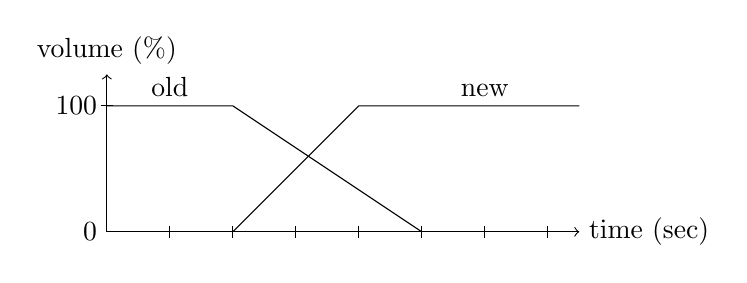
\begin{tikzpicture}[xscale=0.8,yscale=0.8]
\draw[->] (0,0) -- (0,2.5);
\draw (-0.1,2) -- (0.1,2);
\draw (0,2) node[anchor=east]{100};
\draw (0,0) node[anchor=east]{0};
\draw[->] (0,0) -- (7.5,0);
\foreach \x in {1,2,3,4,5,6,7} \draw (\x,-0.1) -- (\x,0.1);
\draw (0,2.5) node[anchor=south]{volume (\%)};
\draw (7.5,0) node[anchor=west]{time (sec)};
\draw (0,2) -- (2,2) -- (5,0);
\draw (2,0) -- (4,2) -- (7.5,2);
\draw (1,2) node[anchor=south]{old};
\draw (6,2) node[anchor=south]{new};
\end{tikzpicture}
\end{center}

\vfill
\pause

\begin{lstlisting}
def mycross(old,new) =
  add([fade.initial(duration=2.,new),
       fade.final(duration=3.,old)])
end

# Apply mycross in between tracks
s = cross(duration=3.,mycross,s)
\end{lstlisting}

\end{frame}

%% ===========================================

\begin{frame}{Features}

\begin{block}{Operators}
\begin{itemize}
\item Play a \kw{single} file, a \kw{playlist} or a queue of files
\item Play a file given by an external script
\item Switch, sequence, add
\item Sound processing: compression, change pitch, etc.
\item Event handlers: tracks, metadata, blank
\item \ldots
\end{itemize}
\end{block}

\begin{block}{Interfaces}
\begin{itemize}
\item Icecast, Shoutcast and compatible: output, relay and host
\item ALSA, OSS, Jack, Pulseaudio, AO\ldots
\end{itemize}
\end{block}

\textbf{Formats:} WAV, Ogg, MP3, AAC+, Flac, external

\textbf{Also}: requests and protocols, server, etc.

\end{frame}

%% ============================================

\begin{frame}{Does it make coffee?}

\pause

\begin{block}{Liquidsoap does not\ldots}
\begin{itemize}
\item No established graphical or web interface, no database stuff
  \\ \emph{But} it can easily communicate with such systems
\item No processing of encoded data
\end{itemize}
\end{block}

\pause

\begin{block}{But what it does, it does it well}
It's even \emph{efficient}:
\begin{itemize}
\item competes with \texttt{ices} on similar tasks
\item 80 instances on a single Core i7 920
\end{itemize}
\end{block}

\end{frame}

% =========================================

\begin{frame}

\vfill\begin{center}
There is more in \\
\LARGE Liquidsoap \emph{1.0} beta
\end{center}\vfill

\end{frame}

\begin{frame}{Stream content}

\begin{center}
\large
  Each source has its own content type: \\
  any number of \textbf{audio video or midi} channels
\begin{flushright}
\small \color{gray} No cost for the user: content types are infered
\end{flushright}
\end{center}

\begin{block}{Traditional radio uses}
\begin{itemize}
\item Manual control over stereo/mono conversions
\item Produce many audio channels ({\em e.g.} dolby) for on-site playout, \\
  convert to stereo for web broadcast
\end{itemize}
\end{block}

\begin{block}{Experimenting}
More ideas to try with video and MIDI\ldots
\end{block}

\end{frame}

%% ===========================================

\begin{frame}{Clocks}

\[
\xymatrix{
  \text{\only<3->{\color{red}}remote server A} \ar[dr] &
        & \mbox{\only<3->{\color{gray}}remote server B} \\
  \text{\only<3->{\color{blue}}soundcard 1} \ar[r]      &
                \text{liquidsoap} \ar[ur]\ar[r]\ar[dr]
        & \mbox{\only<3->{\color{blue}}soundcard 1}     \\
  \text{\only<3->{\color{green}}soundcard 2} \ar[ur] &
        & \mbox{\only<3->{\color{blue}}backup file}
}
\]

\vspace{0.5cm}
\pause

\begin{center}
\large
  A liquidsoap instance can control several clocks, \\
  each source assigned to a single clock
\begin{flushright}
\small \color{gray} No cost for the user: clocks are infered
\end{flushright}
\end{center}

\pause
\pause

%\begin{block}{Uses}
\begin{itemize}
\item Deal with drift and lags of external clocks
\item Avoid internal time inconsistencies (\kw{cross}, \kw{stretch}\ldots)
\end{itemize}
%\end{block}

\end{frame}

%% ===========================================

\begin{frame}{Background}

\begin{block}{The Savonet team}
Open-source development since \emph{2003}, unfunded
\begin{center}
David Baelde, Romain Beauxis and Samuel Mimram \\
Peter Brookes, Vincent Tabard\ldots
\end{center}
Languages: mostly \emph{Ocaml}, also C and various script languages
\end{block}

\vfill

\begin{block}{Community}
\begin{itemize}
\item Not many contributors or even doc writers
\item An established user base (bug reports)
\item Reaching the point where users help each other
\end{itemize}
\end{block}

\end{frame}

%% ===========================================

\begin{frame}{Conclusion}

\begin{block}{Liquidsoap}
\begin{itemize}
\item Many great features
\item A unique ability to combine them at will
\end{itemize}
\end{block}

\begin{block}{Future}
\begin{itemize}
\item Develop uses of video and MIDI streams
\item Coming: more real-time uses, e.g. telephony
\item More fine-grained language, notably for approaching DSP
  % To name a few: chuck, puredata, faust, streamit \ldots
\end{itemize}
\end{block}

\vfill

\begin{center}
  \large \emph{Try liquidsoap, stay tuned, join the community!}
\end{center}

\end{frame}

\end{document}
